\documentclass[a4paper]{article}

%% Language and font encodings
\usepackage[english]{babel}
\usepackage[utf8x]{inputenc}
\usepackage[T1]{fontenc}

%% Sets page size and margins
\usepackage[a4paper,top=3cm,bottom=2cm,left=3cm,right=3cm,marginparwidth=1.75cm]{geometry}

%% Useful packages
\usepackage{amsmath}
\usepackage{graphicx}
\usepackage{textpos}
\usepackage{float}
\usepackage[colorinlistoftodos]{todonotes}
\usepackage[colorlinks=true, allcolors=black]{hyperref}
\usepackage[numbered,framed]{matlab-prettifier}
\usepackage{relsize}
\usepackage{amsmath}
\usepackage{amssymb}
\usepackage{amsthm}

%% Package for graphs
\usepackage{tikz}

%% Package for loading program files
\usepackage{listings}
\usepackage{minted}

%% Package for import verbatim
\usepackage{verbatim}

\setlength{\parindent}{0pt}
\newcommand{\p}{\mathbb{P}}

\title{\vspace*{2cm}9.3 Protein Comparison in Bioinformatics\vspace*{-1.5cm}}
\date{}

\begin{document}
\maketitle

\begin{textblock*}{100mm}(0cm,-5.5cm)
\Huge 9.3
\end{textblock*}

\section*{Introduction}

This project will be investigating sequence comparison and alignment with application to biomolecular sequences of amino acids within proteins and DNA.
%Within this project the following standard notation will be used throughout. We will be comparing strings $S$ and $T$ of lengths $m$ and $n$ respectively. $S_i$ will denote the $i$th character of $S$ and $S[i,j]$ will denote the substring $S_i,\hdots,S_j$. If $i>j$ then $S[i,j]$ is the empty string.

\section*{The Edit Distance}

We define the edit distance $d(S,T)$ to be the minimal number of edits between $S$ and $T$. Define $D$ as follows.
\[ D(i,j) = d(S[1,i],T[1,j]) \]

\subsection*{Question 1}

We prove the following equality for $D(i,j)$, the minimal distance between $S[1,i]$ and $T[1,j]$:
\begin{align}
    \label{eq:q1}
    D(i,j) = min\{ D(i-1,j)+1, D(i,j-1)+1, D(i-1,j-1)+s(S_i,T_i)\}
\end{align}

Given an editing transcript from $S[1,i-1]$ to $T[1,j]$ then simply appending a single deletion, removing $S_i$, creates a transcript from $S[1,i]$ to $T[1,j]$. Thus we have:
\[ D(i,j) \leq D(i-1,j)+1 \]

Similarly for $D(i,j-1)$ except with an insertion, adding $T_j$, rather than a deletion:
\[ D(i,j) \leq D(i,j-1)+1 \]

Given an editing transcript from $S[1,i-1]$ to $T[1,j-1]$ we can form an editing transcript from $S[1,i]$ to $T[1,j]$ by appending a match or replacement depending on whether $S_i$ and $T_j$ match or not. A replacement is an edit operation and so counts towards edit distance while a match does not, this motivates the following form for $s(a,b)$ and a third inequality:
\[ s(a,b) = 1 - \delta_{a,b} = \begin{cases} 0 \qquad a=b \\ 1 \qquad a\neq b \end{cases}\]
\[ D(i,j) \leq D(i-1,j-1)+s(S_i,T_i) \]

Combining the above inequalities we achieve the following:
\begin{align*}
    D(i,j) \leq  min\begin{cases} D(i-1,j)+1 \\ D(i,j-1)+1 \\ D(i-1,j-1)+s(S_i,T_i) \end{cases}
\end{align*}

Suppose $D(i,j)$ were less than the minimum then this would imply that there exists a edit transcript which converts $S$ to $T$ which contradicts the minimality of at least one of $D(i-1,j)$, $D(i,j-1)$ or $D(i-1,j-1)$. Therefore there must be equality giving the desired result. This is further verified by the boundary conditions:
\begin{align*}
    D(0,0) &= 0 \\
    D(i,j) = D(i,0) &= i \quad \forall\ 1 \leq i \leq m,\ j\leq 0 \\
    D(i,j) = D(0,j) &= j \quad \forall\ 1 \leq j \leq n,\ i\leq 0
\end{align*}

\subsection*{Question 2}

Script Q2.py (pg.\pageref{PQ2}) returns the edit distance between two strings entered by the user. The script determines the edit distance between 'shesells' and 'seashells' to be 3 as can be seen in figure \ref{output:q2}.

\begin{figure}[H]
    \centering
    \begin{verbatim}
        Enter a string: shesells
        Enter a string: seashells
        edit distance:  3
    \end{verbatim}
    \caption{Output from Q2.py given input strings "shesells" and "seashells"}
    \label{output:q2}
\end{figure}

The complexity of the algorithm is $O(mn)$ where $m$ and $n$ are the lengths of the first and second strings respectively. This is because the program works by computing values in the distance matrix $D$ where $D_{i,j}=D(i,j)$. At each step $D_{i,j}$ is determined using the values $D_{i-1,j}$, $D_{i,j-1}$ and $D_{i-1,j-1}$ according to equation (\ref{eq:q1}). To determine $D_{m,n} = D(m,n) = d(S,T)$ we therefore require computing the full matrix $D$, that is $(m+1) \times (n+1)$ values. This process is visualised in figure \ref{fig:q2}. Note this is possible because of the boundary conditions.

\begin{figure}[H]
    \centering
    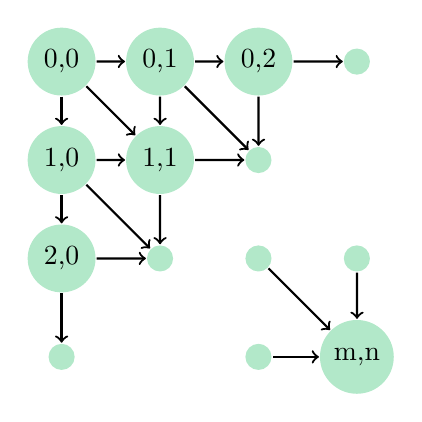
\begin{tikzpicture}
        [scale=1.25,auto=left,thick,every node/.style={circle,fill=blue!30!green!30}]
        \node (00) at (0,3) {0,0};
        \node (10) at (0,2) {1,0};
        \node (20) at (0,1) {2,0};
        \node (30) at (0,0) {};
        \node (01) at (1,3) {0,1};
        \node (11) at (1,2) {1,1};
        \node (21) at (1,1) {};
        \node (02) at (2,3) {0,2};
        \node (12) at (2,2) {};
        \node (03) at (3,3) {};
        
        \path [->] (00) edge (01);
        \path [->] (00) edge (11);
        \path [->] (00) edge (10);
        \path [->] (01) edge (02);
        \path [->] (01) edge (12);
        \path [->] (01) edge (11);
        \path [->] (02) edge (03);
        \path [->] (02) edge (12);
        \path [->] (10) edge (11);
        \path [->] (10) edge (21);
        \path [->] (10) edge (20);
        \path [->] (20) edge (21);
        \path [->] (20) edge (30);
        \path [->] (11) edge (12);
        \path [->] (11) edge (21);
        
        \node (mn) at (3,0) {m,n};
        \node (mn') at (3,1) {};
        \node (m'n) at (2,0) {};
        \node (m'n') at (2,1) {};
        
        \path [<-] (mn) edge (mn'); 
        \path [<-] (mn) edge (m'n); 
        \path [<-] (mn) edge (m'n'); 
    
    \end{tikzpicture}
    \caption{A diagram visualising the dependencies of values in the distance matrix $D$}
    \label{fig:q2}
\end{figure}

\subsubsection*{Question 3}

Script Q3.py (pg.\pageref{PQ3}) produces one optimal vertical alignment between two strings. It is set up to process two myoglobin proteins, A and B, from a duckbill platypus and yellowfin tuna respectively. The script finds the edit distance between these two proteins to be 83, this and the first 50 steps of alignment can be seen in figure \ref{fig:q3}.
\begin{figure}[H]
    \centering
    \begin{verbatim}
        edit distance:  83
        MRRRMRDDDDMMMRMMRMMRMRRRRMRRMMRMMMMRMMMMRDMIMRMMRM
        MGLSDGEWQLVLKVWGKVEGDLPGHGQEVLIRLFKTHPETLEK FDKFKG
        MADFDA    VLKCWGPVEADYTTMGGLVLTRLFKEHPETQ KLFPKFAG
    \end{verbatim}
    \caption{Output from script Q3.py including the edit distance and first 50 steps of an optimal alignment}
    \label{fig:q3}
\end{figure}

\section*{Scoring Matrix}
We will now consider the application to amino acid sequences in DNA proteins. To do this we will make some adjustments to reflect the biological realities of editing protein sequences - different DNA mutations are more or less likely than others. The score function $s$ will be updated to use a BLOSUM matrix as introduced by Henikoff and Henikoff. This will also mean that we will be measuring edit distance as a score to be maximised, rather than a distance to be minimised.

\subsection*{Question 4}
Script Q4.py (pg.\pageref{PQ4}) calculates the score and vertical alignment between proteins A and B according to the new adjusted scoring with BLOSUM matrix with a scoring of insertions and deletions as $-8$. The script calculates a score of 290, this and the first 50 steps of alignment are included in figure \ref{fig:q4}.
\begin{figure}[H]
    \centering
    \begin{verbatim}
        score:  290
        MDDRMDDRRRMMMRMMRMMRMRRRRMRRMMRMMMMRMMMMRRRMRMMRMR
        MGLSDGEWQLVLKVWGKVEGDLPGHGQEVLIRLFKTHPETLEKFDKFKGL
        M  AD  FDAVLKCWGPVEADYTTMGGLVLTRLFKEHPETQKLFPKFAGI
    \end{verbatim}
    \caption{Output from script Q4.py including the score and first 50 steps of the optimal alignment}
    \label{fig:q4}
\end{figure}

\section*{Scoring for gaps}

Some mechanisms for DNA mutation allow for the insertion or deletion of large chunks of DNA. We therefore develop our scoring system as follows. Let $w(l)$ be the score of inserting/deleting a sequence of amino acids of length $l$. Let $v_{gap}(S,T)$ be the gap-weighted score between $S$ and $T$.

\subsection*{Question 5}

It is possible to determine $v_{gap}$ with an algorithm of complexity $O(mn)$. To see this we firstly observe the following:
\begin{align*}
    E(i,j) &= \underset{0\leq k\leq j-1}{max} \big\{ \ V_{gap}(i,k) + w(j-k) \ \big\} \\
        `  &= max \big\{ \ \underset{0\leq k\leq j-2}{max} \{ V_{gap}(i,k) + w(j-k) \} \ , \ V_{gap}(i,j-1) + w(1) \ \big\} \\
           &= max \big\{ \ E(i,j-1) \ , \ V_{gap}(i,j-1) + w(1) \ \big\}
\end{align*}
Similarly for $D$:
\[ D(i,j) = max \big\{ \ D(i-1,j) \ , \ V_{gap}(i-1,j) + w(1) \ \big\} \]
Computing $E$ and $D$ according to these formulae reduces the complexity for calculating $E(i,j)$ and $D(i,j)$ from $O(i)$ and $O(j)$ respectively to $O(1)$.

\bigskip
Due to the interdependence of the matrices, in order to determine $V_{gap}(m,n)$ we require calculating the entirety of all three matrices similarly to Questions 1. We can achieve this by iterating through the $m\times n$ grid as follows:

\bigskip
Start by computing $V_{gap}(1,1)$ which is possible from the boundary conditions alone. Then iterate though the points on the $m \times n$ grid in columns. At each point $(i,j)$ compute $V_{gap}(i,j)$ and then the following dependant values: $E(i,j+1)$, $F(i+1,j)$ and $G(i+1,j+1)$. These new values will enable the process to progress to $(i+1,j)$ and compute $V_{gap}(i+1,j)$. At the end of each column, $(m,j)$, continue from from $(1,j+1)$. 

\bigskip
Iterating over the $n \times m$ grid has complexity $O(mn)$, the calculations at each point are $O(1)$ and so the overall complexity of this algorithm is $O(mn)$.

\subsubsection*{Boundary Conditions}
Here we describe the boundary conditions referenced above. Firstly, for $V_{gap}$, we have the following conditions based on the restriction that transforming to/from an empty string permits only delete/insert operations. Since $w(l)=u$, a negative constant, deletion/insertion is most effectively done in single edits giving a score of $u$.

\begin{figure}[H]
    \centering
    \begin{minipage}{0.35\textwidth}
        \centering
        \begin{align*}
            V_{gap}(0,0) &= 0 \\
            V_{gap}(i,0) &= u \quad \forall\ 1 \leq i \leq m \\
            V_{gap}(0,j) &= u \quad \forall\ 1 \leq j \leq n
        \end{align*}
    \end{minipage}
    \begin{minipage}{0.35\textwidth}
        \centering
        \begin{align*}
            V_{gap} = \begin{pmatrix}
                            0 & u & \hdots & u \\
                            u \\
                            \vdots \\
                            u
                      \end{pmatrix}
        \end{align*}
    \end{minipage}
\end{figure}


Based on the boundary conditions for $V_{gap}$ we can extend to boundary conditions on $E$, $F$ and $G$ according to their definitions. The following conditions hold for all $1 \leq i \leq m,\ 1 \leq j \leq n$.
\begin{figure}[H]
    \centering
    \begin{minipage}{0.3\textwidth}
        \centering
        \begin{align*}
            E(i,1) &= 2u \\
            E(0,j) &= u
        \end{align*}
    \end{minipage}
    \begin{minipage}{0.3\textwidth}
        \centering
        \begin{align*}
            E = \begin{pmatrix}
                \times & u & u & \hdots & u \\
                \times & 2u \\
                \vdots & \vdots \\
                \times & 2u
            \end{pmatrix}
        \end{align*}
    \end{minipage}
\end{figure}
\begin{figure}[H]
    \centering
    \begin{minipage}{0.3\textwidth}
        \centering
        \begin{align*}
            F(i,0) &= u \\
            F(1,j) &= 2u
        \end{align*}
    \end{minipage}
    \begin{minipage}{0.3\textwidth}
        \centering
        \begin{align*}
            F = \begin{pmatrix}
                \times & \times & \hdots & \times \\
                u & 2u & \hdots & 2u \\
                \vdots \\
                u
            \end{pmatrix}
        \end{align*}
    \end{minipage}
\end{figure}
\begin{figure}[H]
    \centering
    \begin{minipage}{0.48\textwidth}
        \centering
        \begin{align*}
            Q(i,1) &= V_{gap}(i-1,0) + s(S_i,T_1) \\
                   &= u + s(S_i,T_1) \\
            Q(1,j) &= V_{gap}(0,j-1) + s(S_1,T_j) \\
                   &= u + s(S_1,T_j)
        \end{align*}
    \end{minipage}\hfill
    \begin{minipage}{0.48\textwidth}
        \centering
        \begin{align*}
            Q = \begin{pmatrix}
                \times & \times & \hdots & \times \\
                \times & u+s(S_1,T_1) &\hdots & u+s(S_1,T_n) \\
                \vdots & \vdots \\
                \times & u+s(S_m,T_1)
            \end{pmatrix}
        \end{align*}
    \end{minipage}
\end{figure}

Note: we don't need the following values for any of the computations so we can ignore these values, in the matrices above they have been marked by a $\times$.
\begin{align*}
    E(i,0),\ G(i,0) \quad \forall \ 1 \leq i \leq m \\
    F(0,j),\ G(0,j) \quad \forall \ 1 \leq j \leq n \\
\end{align*}

\subsection*{Question 6}

Script Q6.py (pg.\pageref{PQ6}) applies the algorithm from question 5 to proteins C and D with insertion/deletion score $u=12$. The gap-weighted score between these two proteins is 305, this and the first 50 steps of alignment are included in figure \ref{fig:q6}.

\begin{figure}[H]
    \centering
    \begin{verbatim}
        gap-wegihted score:  305
        MDDDDRRRRRMMMRMMRMMRMRRRRMRRMMRMMMMRMMMMRRRMRMMRMR
        MGLSDGEWQLVLKVWGKVEGDLPGHGQEVLIRLFKTHPETLEKFDKFKGL
        M    ADFDAVLKCWGPVEADYTTMGGLVLTRLFKEHPETQKLFPKFAGI
    \end{verbatim}
    \caption{Output from script Q6.py including the gap-weighted score and first 50 steps of the optimal alignment}
    \label{fig:q6}
\end{figure}

\section*{Statistical significance}
We now investigate at what threshold a score $v_{gap}(S,T)$ should be declared to have biological significance.

\subsection*{Question 7}
Let $U^n$ and $V^n$ be random proteins on length $n$ made up of only two amino acids, $a$ and $b$, with a probability, $p$, that any given amino acid is $a$. We start by considering a loose lower bound on $\mathbb{E}(v_{gap}(U,V))$ using only match and replace operations:
\begin{align*}
    \mathbb{E}(v_{gap}(U,V)) &= \sum_{u=a,b} \sum_{v=a,b} \mathbb{P}(U=u,V=v) \times s(u,v) \\
                             &= \mathbb{P}(U=a,V=a) \times s(a,a) + \mathbb{P}(U=a,V=b) \times s(a,b) \\
                             &\quad + \mathbb{P}(U=b,V=a) \times s(b,a) + \mathbb{P}(U=b,V=b) \times s(b,b)\\
                             &= p^2 - p(1-p) -(1-p)p + (1-p)^2 \\
                             &= (1-2p)^2 \\
                             &\geq 0
\end{align*}

We now observe the following inequality:
\begin{align*}
     v_{gap}(U^n,V^n) \geq v_{gap}(U^{n-1},V^{n-1}) + v_{gap}(U_n,V_n)
\end{align*}
This holds because any valid edit transcripts for $U^{n-1}$ to $V^{n-1}$ and $U$ to $V$ can be concatenated to make a valid edit transcript for $U^n$ to $V^n$. However, a valid edit transcript from $U^n$ to $V^n$ may not be separable into two transcripts for $U^{n-1}$ to $V^{n-1}$ and $U$ to $V$ because it may use a multi-insert/delete which spans the break between the two sub-sequences. Applying this result repeatedly we find:
\begin{align*}
     v_{gap}(U^n,V^n) &\geq v_{gap}(U^{n-1},V^{n-1}) + v_{gap}(U_n,V_n) \\
                      &\geq v_{gap}(U^{n-2},V^{n-2}) + v_{gap}(U_{n-1},V_{n-1}) + v_{gap}(U_n,V_n) \\
                      &\geq \qquad \vdots \\
                      &\geq \sum_{i=1}^n v_{gap}(U_i,V_i)
\end{align*}
Taking expectation we continue:
\begin{align}\label{eq7a}
\begin{split}
     \mathbb{E}(v_{gap}(U^n,V^n)) &\geq \mathbb{E}\big(\sum_{i=1}^n v_{gap}(U_i,V_i)\big) \\
                                  &\geq \sum_{i=1}^n \mathbb{E}(v_{gap}(U_i,V_i)) \\
                                  &\geq \sum_{i=1}^n (1-2p)^2 \\
                                  &\geq n(1-2p)^2
\end{split}
\end{align}

We now consider the insertion and deletion operations. We seek to show that for sufficiently long sequences we can improve the lower bound described above. For a sequence of length $n$, $s^n$, let us define an anti-sequence, $\overline{s^n}$, as a sequence with $s^n_i \neq \overline{s^n}_i \quad \forall\ 1\leq i\leq n$.

\bigskip
Consider some sequence $s^n$. Using the previous method of bounding using only match and replace operations, in this case only replace operations, we have:
\begin{align}\label{eq7b}
    v_{gap}(s^n, \overline{s^n}) \geq -n
\end{align}
However, with the insert/delete operations we can introduce a second bound based on a simple editing transcript of one delete operation, to remove the entirety of $s^n$, and one insert operation, to add the entirety of $\overline{s^n}$.
\begin{align}\label{eq7c}
    v_{gap}(s^n, \overline{s^n}) &\geq 2u
\end{align}
Therefore, in the case that $n\geq -2u$ then this second lower bound improves upon the first.

\bigskip
In this question we consider an alphabet of only 2 amino acids, so for each sequence that $U^n$ can take there is exactly one sequence $V^n$ can take which will be an anti-sequence. Noting that by construction a sequence and anti-sequence must in total contain an equal number of a's and b's we reach the following:
\begin{align*}
    \mathbb{P}(U^n = \overline{V^n}) = 2^n \times p^n (1-p)^n
\end{align*}

Let $N$ be an integer such that $u>-N$. We now consider the case of two sequences $U^n$ and $V^n$ with $n=m(2N+1)$ for some integer $m$. We can then partition the sequences into a series of subsequences of length $2N+1$ and use the improved lower bound involving insert/delete operations, as described above in equations \ref{eq7b} and \ref{eq7c}, to improve the expected score.
\begin{align*}
     \mathbb{E}(v_{gap}(U^n, V^n)) &\geq m \times \mathbb{E}(v_{gap}(U^{2N+1}, V^{2N+1})) \\
                                   &\geq m \bigg( (2N+1)(1-2p)^2 + ((2N+1) - 2u)[2p(1-p)]^{2N+1} \bigg)
\end{align*}
Where the first term comes derives from equation \ref{eq7a} and the second term is the improvement in lower bound for sequence and anti-sequence pairs. Rearranging we then get:
\begin{align*}
     \mathbb{E}(v_{gap}(U^n, V^n)) &\geq m \bigg( (2N+1)(1-2p)^2 + [2p(1-p)]^{2N+1} \bigg) \\
                                   &\geq n \bigg( (1-2p)^2 + \frac{[2p(1-p)]^{2N+1}}{2N+1} \bigg)
\end{align*}
Dividing by $n$ we then see we have found a positive lower bound independent of $n$:
\begin{align*}
     \frac{\mathbb{E}(v_{gap}(U^n, V^n))}{n} &\geq (1-2p)^2 + \frac{[2p(1-p)]^{2N+1}}{2N+1} > 0 \qquad \forall\ 0\leq p \leq 1
\end{align*}
Therefore, taking $n\rightarrow\infty$ by taking $m\rightarrow\infty$ we conclude that for all $0\leq p \leq 1$ and for all $u\leq0$:
\begin{align*}
    \liminf_{n\rightarrow\infty} \frac{\mathbb{E}(v_{gap}(U^n,V^n))}{n} &\geq 0
\end{align*}

\subsection*{Question 8}
Script Q8.py (pg.\pageref{PQ8}) estimates $n^{-1}\mathbb{E}(v_{gap}(U^n,V^n))$ with $u=-3$ and $p=\frac{1}{2}$ for a specified $n$. Figure \ref{fig:q8} includes output for a selection of $n$ values. From this data the we can then make the further estimate that the limit of $n^{-1}\mathbb{E}(v_{gap}(U^n,V^n))$ looks to be tending towards $\approx 0.45$.
\begin{figure}[H]
    \centering
    \begin{verbatim}
         n     estimate
        ____   ________
         100   0.3560
         500   0.4240
        1000   0.4264
        1500   0.4328
        2000   0.4366
        3000   0.4390
    \end{verbatim}
    \caption{Estimations of $n^{-1}\mathbb{E}(v_{gap}(U^n,V^n))$ (right) for increasing values of $n$ (left).}
    \label{fig:q8}
\end{figure}

\section*{Local Alignment}

\subsection*{Question 9}
In the study of DNA it can be helpful to identify highly conserved regions between two closely related DNA sequences. This motivates the definition:
\begin{align*}
    v_{sub}(S,T) = max\big\{ v(S',T') &: S' \text{ a substring of } S,\ T' \text{ a substring of } T \big\}
\end{align*}
We find that $v_{sub}(S,T)$ can be expressed in the following form:
\begin{align}\label{eq:q9}
    v_{sub}(S,T) = max\big\{ v_{sfx}(S',T') &: S' \text{ a prefix of } S,\ T' \text{ a prefix of } T \big\}
\end{align}
To prove equation (\ref{eq:q9}) it is helpful to recall the definition of $v_sfx$ and observe:
\begin{align*}
    v_{sfx}(S,T) &= max\big\{ v(S',T') : S' \text{ a suffix of } S,\ T' \text{ a suffix of} T \big\} \\
                 &= max\big\{ v(S[i:m],T[k:n]) : 1\leq i\leq m,\ 1\leq k\leq n \big\}
\end{align*}
We can now prove equation (\ref{eq:q9}) as follows:
\begin{align*}
        max\big\{ v_{sfx}(S',T') &: S' \text{ a prefix of } S,\ T' \text{ a prefix of } T \big\} \\
        &= max\big\{ v_{sfx}(S[1:j],T[1:l]) : 1\leq j\leq m, 1\leq l\leq n \big\} \\
        &= max\Big\{ max\big\{ v(S[i:j],T[k:l]) : 1\leq i\leq j,\ 1\leq k\leq l \big\} : 1\leq j\leq m,\ 1\leq l\leq n \Big\} \\
        &= max\big\{ v(S[i:j],T[k:l]) : 1\leq i\leq j\leq m,\ 1\leq k \leq l\leq n \big\} \\
        &= max\big\{ v(S',T') : S' \text{ a substring of } S,\ T' \text{ a substring of } T \big\} \\
        &= v_{sub}(S,T)
\end{align*}

\subsection*{Question 10}

To prove equation (\ref{eq:q10}) we observe similarities between $V_{sfx}$ and $D$ and so apply a similar logic.
\begin{align}\label{eq:q10}
    V_{sfx}(i,j) &= max
    \begin{cases}
        0 \\
        V_{sfx}(i-1,j-1) + s(S_i,T_j) \\
        V_{sfx}(i-1,j) + s(S_i,-) \\
        V_{sfx}(i,j-1) + s(-,T_j) \\
    \end{cases}
\end{align}

$V_{sfx}(i,j)$ is at least $0$ because it is always possible to take both suffixes to be zero-length strings which trivially score 0.
\[ V_{sfx}(i,j) \geq 0 \]

Given an editing transcript from a suffix pf $S[1,i-1]$ to a suffix of $T[1,j-1]$ we note that adding an edit operation between $S_i$ and $T_j$ produces an editing transcript from a suffix of $S[1,j]$ to a suffix of $T[1,j]$.
\[ V_{sfx}(i,j) \geq V_{sfx}(i-1,j-1) + s(S_i,T_j) \]

Similarly for $V_{sfx}(i-1,j)$ and $V_{sfx}(i,j-1)$ we have that their editing transcripts can be extended while maintaining the property of being transcripts between two suffixes.
\begin{align*}
    V_{sfx}(i,j) &\geq V_{sfx}(i-1,j) + s(S_i,-) \\
    V_{sfx}(i,j) &\geq V_{sfx}(i,j-1) + s(-,S_j)
\end{align*}

Combining the above inequalities and observing that $V_{sfx}(i,j)$ taking any value greater than this would lead to a contradiction with the maximality of at least one other $V_{sfx}$ we achieve the desired result.

\subsection*{Question 11}

We can determine $v_{sub}$ by calculating $V_{sfx}(i,j)$ for all $0\leq i\leq m$, $0\leq j \leq n$ and then finding the maximum by equation \ref{eq:q9}. Script Q11.py (pg.\pageref{PQ11}) is an adaptation of Q4.m in order to achieve this. Applying this script we find $v_{sub}=1312$ (figure \ref{fig:q11}).

\begin{figure}[H]
    \centering
    \begin{verbatim}
        v_sub =  1312
    \end{verbatim}
    \caption{Output of $v_{sub}$ as calculated by script Q11.py.}
    \label{fig:q11}
\end{figure}

\pagebreak
\section*{Programs}

\subsection*{Q2.py}\label{PQ2}
\inputminted[frame=single,linenos,framesep=2mm,baselinestretch=1]{python}{Q2.py}

\pagebreak
\subsection*{Q3.py}\label{PQ3}
Dependencies: data.py (pg.\pageref{Pdata})
\inputminted[frame=single,linenos,framesep=2mm,baselinestretch=1]{python}{Q3.py}

\pagebreak
\subsection*{data.py}\label{Pdata}
\inputminted[frame=single,linenos,framesep=2mm,baselinestretch=1]{python}{data.py}


\pagebreak
\subsection*{Q4.py}\label{PQ4}
Dependencies: Q3.py (pg.\pageref{PQ3}), data.py (pg.\pageref{Pdata})
\inputminted[frame=single,linenos,framesep=2mm,baselinestretch=1]{python}{Q4.py}

\subsection*{Q5.py}\label{PQ5}
Dependencies: Q3.py (pg.\pageref{PQ3})
\inputminted[frame=single,linenos,framesep=2mm,baselinestretch=1]{python}{Q5.py}

\subsection*{Q6.py}\label{PQ6}
Dependencies: Q5.py (pg.\pageref{PQ5}), data.py (pg.\pageref{Pdata})
\inputminted[frame=single,linenos,framesep=2mm,baselinestretch=1]{python}{Q6.py}

\newpage
\subsection*{Q8.py}\label{PQ8}
Dependencies: Q5.py (pg.\pageref{PQ5})
\inputminted[frame=single,linenos,framesep=2mm,baselinestretch=1]{python}{Q8.py}

\newpage
\subsection*{Q11.py}\label{PQ11}
Dependencies: data.py (pg.\pageref{Pdata})
\inputminted[frame=single,linenos,framesep=2mm,baselinestretch=1]{python}{Q11.py}


% \pagebreak
% \section*{Appendix}

% \subsection*{Proteins}
% \subsubsection*{II-9-3-2018-proteins.txt}
% \verbatiminput{II-9-3-2018-proteins.txt}

% \pagebreak
% \subsection*{Blosum Matrix}
% \subsubsection*{II-9-3-2018-blosum.txt}
% \verbatiminput{II-9-3-2018-blosum.txt}

\end{document}
